\documentclass{article}

% http://bayesiandeeplearning.org/
% if you need to pass options to natbib, use, e.g.:
% \PassOptionsToPackage{numbers, compress}{natbib}
% before loading nips_2018

% ready for submission
\usepackage[nonatbib,final]{nips_2018}

% to compile a preprint version, e.g., for submission to arXiv, add
% add the [preprint] option:
% \usepackage[preprint]{nips_2018}

% to compile a camera-ready version, add the [final] option, e.g.:
% \usepackage[final]{nips_2018}

% to avoid loading the natbib package, add option nonatbib:
% \usepackage[nonatbib]{nips_2018}

\usepackage[utf8]{inputenc} % allow utf-8 input
\usepackage[T1]{fontenc}    % use 8-bit T1 fonts
\usepackage{hyperref}       % hyperlinks
\usepackage{url}            % simple URL typesetting
\usepackage{booktabs}       % professional-quality tables
\usepackage{amsmath}
\usepackage{amsfonts}       % blackboard math symbols
\usepackage{nicefrac}       % compact symbols for 1/2, etc.
\usepackage{microtype}      % microtypography
\usepackage{graphicx}
\usepackage{subcaption}
\usepackage{booktabs}
\usepackage{siunitx}

\usepackage[numbers]{natbib}

% TODO should we make network plural or not??
\title{Metropolis-Hastings\\Generative Adversarial Networks}

% The \author macro works with any number of authors. There are two
% commands used to separate the names and addresses of multiple
% authors: \And and \AND.
%
% Using \And between authors leaves it to LaTeX to determine where to
% break the lines. Using \AND forces a line break at that point. So,
% if LaTeX puts 3 of 4 authors names on the first line, and the last
% on the second line, try using \AND instead of \And before the third
% author name.

\author{
  Ryan Turner \\
  Uber AI Labs
  \And
  Jane Hung \\
  Uber AI Labs
  \And
  Jason Yosinski \\
  Uber AI Labs
  \And
  Yunus Saatci \\
  Uber AI Labs
}

\renewcommand{\vec}[1]{{\boldsymbol{\mathbf{#1}}}} % vector
\newcommand{\mat}[1]{{\ensuremath{\mathbf{#1}}}} % matrix

\newcommand{\R}{\mathbb{R}}
\newcommand{\D}{\mathcal{D}}
\newcommand{\N}{\mathcal{N}}
\newcommand{\set}[1]{\mathcal{#1}}

\newcommand{\bigO}{\mathcal{O}}
\newcommand{\ceq}{{\stackrel{c}{=}}}
\newcommand{\half}{\frac{1}{2}}
\newcommand{\T}{^\top}
\newcommand{\I}{\mathbb{I}}

\newcommand{\grad}{\nabla}
\newcommand{\sample}{\sim}
\newcommand{\given}{|}

\newcommand{\norm}{\mathcal{N}}
\newcommand{\bern}{\textrm{Bern}}

\DeclareMathOperator*{\argmin}{argmin}
\DeclareMathOperator*{\argmax}{argmax}

\newcommand{\target}{{p^\star}}
\newcommand{\prop}{q}
\newcommand{\pinit}{{p_0}}

\newcommand{\PG}{{p_G}}
\newcommand{\PD}{{p_D}}
\newcommand{\PR}{{p_{\textrm{data}}}}
\newcommand{\accept}{\alpha}

\newcommand{\setx}{\set{X}}

% Typical finish clean up checks:
% use smash where needed
% \! arrow where needed
% search for: can overuse, It is ...

% TODO add lemma

\begin{document}
% \nipsfinalcopy is no longer used

\maketitle

\begin{abstract}
We introduce the Metropolis-Hastings Generative Adversarial Network (MH-GAN), which combines aspect of Markov chain Monte Carlo and GANs.
The MH-GAN samples from the distribution implicitly defined by the generator in a GAN\@.
As such it uses the discriminator from GAN training to build a wrapper around the generator for improved sampling.
With a perfect discriminator, this wrapped generator samples from the true distribution on the data exactly.
We demonstrate results on common GAN data sets and wrap the popular DCGAN and WGAN\@.
\end{abstract}

\section{Introduction}

% GANs provide implicit way to do density estimation
Traditionally, density estimation is done with a model that can compute the data likelihood.
Generative adversarial networks (GANs)~\citep{Goodfellow2014} present a radically new way to do density estimation:
They implicitly represent the density of the data via a classifier that distinguishes real from generated data.
Computing the likelihood has been at least as easy as sampling new data from the trained model.
GANs turn this paradigm on its head.

% GAN uses D and G, but then D usually thrown away => use new method to capture knowledge captured in D, to wrap G and create a more intelligent G'
GANs iterate between updating a discriminator $D$ and a generator $G$, where $G$ generates new (synthetic) samples of data, and $D$ attempts to distinguish samples of $G$ from the real data.
In the typical setup, $D$ is thrown away at the end of training, and only $G$ is kept for generating new synthetic data points.
In this work we propose the Metropolis-Hastings GAN (MH-GAN), a GAN that constructs a new generator $G'$ that ``wraps'' $G$ using the information contained in $D$.
This principle is illustrated in Figure~\ref{fig:block_diag}.

% Assume D is bayes optimal
The MH-GAN uses Markov chain Monte Carlo (MCMC) methods to sample from the distribution implicitly defined by the discriminator $D$ learned for the generator $G$.
This is built upon the notion that the discriminator classifies between the generator $G$ and a data distribution:
\begin{align}
  D(\vec x) = \frac{\PD(\vec x)}{\PD(\vec x) + \PG(\vec x)} \,, \label{eq:define PD}
\end{align}
where $\PG$ is the (intractable) density of samples from the generator $G$, and $\PD$ is the data density \emph{implied} by the discriminator $D$.
If GAN training reaches its global optimum then this discriminator distribution $\PD$ is equal to the true distribution on the data ($\PR = \PD$)~\citep{Goodfellow2014}.

% MCMC only needs the ratio of \PR/G and this can be found from D
We use an MCMC \emph{independence sampler}~\citep{Tierney1994} to get samples from $\PD$ using multiple samples from $G$ (as the proposal)\@.
A corollary is that given a perfect discriminator $D$ and a decent (but imperfect) generator $G$, we can obtain exact samples from the true data distribution $\PR$.
Standard MCMC implementations require (unnormalized) densities for the target $\PD$ and the proposal $\PG$, which are both unavailable for GANs.
Neither of these quantities are available in GANs.
However, the MH algorithm requires only the ratio
\begin{align}
  \frac{\PD(\vec x)}{\PG(\vec x)} = \frac{D(\vec x)}{1 - D(\vec x)}\,, \label{eq:PD inv}
\end{align}
which only requires us to evaluate $D(\vec x)$.

\begin{figure}[bhtp]
    \centering
    \begin{subfigure}[t]{2.25in}
       \centering
       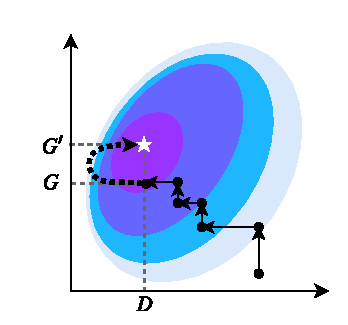
\includegraphics[scale=1.0]{figures/coord_descent.pdf}
       \caption{GAN objective}
    \end{subfigure}
    \hfill
    \begin{subfigure}[t]{3in}
       \centering
       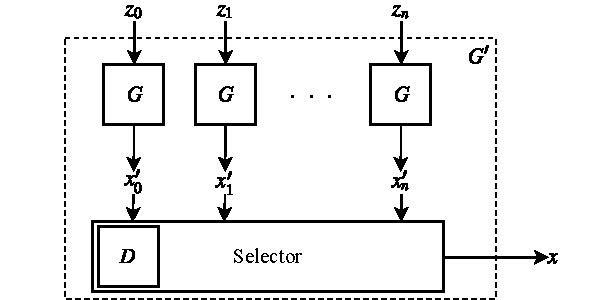
\includegraphics[scale=1.0]{figures/block_diag.pdf}
       \caption{$G'$ wraps $G$}
    \end{subfigure}
    \caption{{\small
    On the left, we illustrate how training of $D$ and $G$ in GANs performs coordinate descent on the joint minimax objective, shown in the solid black arrow.
    If GAN training produces a perfect $D$ for an imperfect $G$, the MH-GAN wraps $G$ to produce a perfect generator $G'$, as shown in the final dashed arrow.
    On the right, we illustrate how the MH-GAN is essentially a selector from multiple draws of $G$.
    In the MH-GAN, the selector is built using a Metropolis-Hastings (MH) acceptance rule from the discriminator scores $D$.
    }}
    \label{fig:block_diag}
\end{figure}

The outline of this paper is as follows:
Section~\ref{sec:Related Work} reviews diverse areas of relevant prior work.
In Sections~\ref{sec:MCMC Methods} and~\ref{sec:GANs} we explain the necessary background on MCMC methods and GANs.
We explain our methodology of combing these two very different areas in Section~\ref{sec:Methods}; here we derive the wrapped generator $G'$.
Results on real data (CIFAR-10 and CelebA) and extending widespread GAN models (DCGAN and WGAN) are shown in Section~\ref{sec:Results}.
Section~\ref{sec:conclusions} discusses implications and conclusions.

\section{Related Work}
\label{sec:Related Work}

% Need to be clear on diff with NICE-MCMC
A few other works combine GANs and MCMC in some way.
\citet{Song2017} use a GAN-like procedure to train a RealNVP~\citep{Dinh2016} MCMC proposal for sampling an externally provided target \smash{$\target$}.
While \citet{Song2017} use GANs to accelerate MCMC, we use MCMC to enhance the samples from a GAN\@.
Similar to \cite{Song2017}, \citet{Kempinska2017} improve proposals in particle filters rather than MCMC\@.
\citet{Song2017} was recently generalized by~\citet{Neklyudov2018}.

% DRE analogy
The GAN approach to density estimation is complementary to the lesser known \emph{density ratio estimation}~\citep{Sugiyama2012} (DRE)\@.
In DRE the generator $G$ is fixed and the density is found by combining Bayes' rule and the learned classifier $D$.
In GANs, the key is learning $G$ well; while in DRE the key is learning $D$ well.
The MH-GAN has flavors of both in that it uses both $G$ and $D$ in $G'$.

% Diff to Google DRS work
A very similar concurrent work is that of \citet{Azadi2018}, who propose discriminator rejection sampling (DRS) for GANs: performing rejection sampling of outputs of $G$ by using the probabilities given by $D$.
This approach is conceptually simpler at first, but suffers from two major shortcomings in practice.
First, it is necessary to find an upper-bound on $D$ over all possible samples (i.e., a valid proposal distribution for rejection sampling)\@.
Because this is not possible, one must instead rely on trying to crudely estimate this proposal by drawing many pilot samples.
Secondly, even if one were to find a good proposal, due to the high-dimensionality of the sampling space, the acceptance rate becomes very low, which leads~\citet{Azadi2018} to use an extra $\gamma$ heuristic to shift the logit $D$ scores; this makes the model sample from a distribution different from $\PR$ even when $D$ is perfect.
We use MCMC instead, which was invented precisely as a replacement for rejection sampling in higher dimensions.
We further improve the robustness of MCMC via use of a \emph{calibrator} on the discriminator to get more accurate probabilities for computing acceptance probabilities.

\section{Background and Notation}
\label{sec:Background}

\subsection{MCMC Methods}
\label{sec:MCMC Methods}

MCMC methods attempt to draw a chain of samples $\vec x_{1:K} \in \setx^K$ that marginally come from a target distribution $\target$.
We refer to the initial distribution as $\pinit$ and the proposal for the independence sampler as $\vec x' \sample \prop(\vec x' \given \vec x_k)=\prop(\vec x')$.
The proposal $\vec x' \in \setx$ is accepted with probability
\begin{align}
  \accept(\vec x', \vec x_k) = \min\left(1, \frac{\target(\vec x')\prop(\vec x_k)}{\target(\vec x_k)\prop(\vec x')}\right) \in [0,1]\,. \label{eq:alpha def}
\end{align}
If $\vec x'$ is accepted, $\vec x_{k+1} = \vec x'$, otherwise $\vec x_{k+1} = \vec x_k$.
Note that when estimating the distribution on $\target$ one must include the duplicates that are a result of rejections in $\vec x'$.

Each chain samples $\vec x_0 \sample \pinit$ and then does $K$ MH iterations to get $\vec x_K$ as the output of $G'$.
That is, $\vec x_K$ is the output of $G'$: Each MCMC chain results in a single sample for $G'$.
Independent chains are used for multiple samples from $G'$.

The detailed balance condition implies that if $\vec x_k \sample \target$ exactly then $\vec x_{k+1} \sample \target$ exactly as well.
Additionally, even if $\vec x_k$ is not exactly distributed according to $\target$, its KL divergence to $\target$ will always decrease as $k$ increases~\citep{Murray2008,Cover2012}.
Note that the number of samples $K$ is meant to be ancillary to the state of the Markov chain $\vec x_k$.
Using the state of the Markov chain to determine when to stop has the potential to introduce bias~\citep{Cowles1999}.

\subsection{GANs}
\label{sec:GANs}

GANs implicitly model the data $\vec x$ via a synthetic data generator \smash{$G \in \R^{d} \rightarrow \setx$}: \smash{$\vec x = G(\vec z)$}, \smash{$\vec z \sample \norm(\vec 0, \vec I_{d})$}.
This implies a (intractable) distribution on the data $\vec x \sample \PG$.
We refer to the unknown true distribution on the data $\vec x$ as $\PR$.
The discriminator $D \in \setx \rightarrow [0,1]$ is a soft classifier predicting if a data point is real (as opposed to being sampled from $\PG$)\@.
% TODO break back out into eqn form
If $D$ converges optimally for a fixed $G$, then \smash{$D = \PR/(\PR + \PG)$}, and if both $D$ and $G$ converge then $\PG = \PR$~\citep{Goodfellow2014}.
GAN training forms a game between $D$ and $G$.
In practice $D$ is often better at estimating the density ratio than G is at generating high-fidelity samples~\citep{Shibuya2017}.
This motivates wrapping an imperfect $G$ to obtain an improved $G'$ by using a more advanced $D$.

\section{Methods}
\label{sec:Methods}

% Derive basic trick for MCMC using D
In this section we show how to sample from the distribution $\PD$ implied by the discriminator $D$.
If we assume that $D$ is a Bayes' discriminator between the generator $\PG$ and \emph{some} alternative distribution $\PD$ as per~\eqref{eq:PD inv}, we can apply~\eqref{eq:alpha def} for a target of $\target=\PD$ and proposal $\prop=\PG$:
\begin{align}
  \frac{\PD}{\PG} = \frac{1}{D^{-1} - 1} \implies
  \accept(\vec x', \vec x_k) = \min\left(1, \frac{D(\vec x_k)^{-1} - 1}{D(\vec x')^{-1} - 1}\right)\,. \label{eq:alpha from D}
\end{align}
If $D$ is perfect, $\PD = \PR$.
The ratio $\PD/\PG$ is computed entirely from the discriminator scores $D$.

\paragraph{Calibration}
The probabilities for $D$ must not merely provide a good AUC score, but must be well \emph{calibrated}.
Put in other terms, if one were to warp the probabilities of the perfect discriminator in~\eqref{eq:define PD} it may still suffice for standard GAN training, but it will not work in the MCMC procedure defined in~\eqref{eq:alpha from D}.

To calibrate $D$, we use a \emph{held out} calibration set and either logistic, isotonic, or beta~\citep{Kull2017} regression to warp the output of $D$.
Furthermore, for WGAN, calibration is required as it does not learn a typical GAN probabilistic discriminator.

We also detect miscalibration of $D$ using the statistic of~\citet{Dawid1997} on held out samples $\vec x_{1:N}$ and real/fake labels $y_{1:N} \in \{0,1\}^N$.
If $D$ is well calibrated, i.e., $y$ is indistinguishable from a $y \sample \bern(D(\vec x))$,
\begin{align}
  Z := \frac{\sum_{i=1}^N y_i - D(\vec x_i)}{\sqrt{\sum_{i=1}^N D(\vec x_i) (1 - D(\vec x_i))}} \in \R \implies Z \sample \norm(0,1)\,.
  \label{eq:calib score}
\end{align}
This means that large magnitude values for $Z$, i.e., ($|Z| > 2$), reject the hypothesis that $D$ is well-calibrated.

\paragraph{Initialization}
We also avoid the burn-in issues that usually plague MCMC methods.
Recall that via the detailed balance property~\citep[Ch.~1]{Gilks1996}, if the marginal distribution of a Markov chain state $\vec x \in \setx$ at time step $k$ matches the target $\PD$ (\smash{$\vec x_k \sample \PD$}), then the marginal at time step $k+1$ will also follow $\PD$ (\smash{$\vec x_{k+1} \sample \PD$})\@.
In most MCMC applications it is not possible to get an initial sample from the target distribution (\smash{$\vec x_0 \sample \PD$})\@.
However, in MH-GANs, we are sampling from the \emph{data} distribution, so we may use a trick:
Initialize the chain at a sample of real data (the correct distribution) to avoid burn-in.
If not a single generated sample is accepted, we restart sampling from a synthetic sample to ensure the initial real sample is never output.
To make these restarts rare, we set $K$ large (often 640)\@.

% Note how requirement not that strong with calib and manifold
\paragraph{Perfect Discriminator}
The assumption of perfect $D$ may be weakened for two reasons:
(A)~Because we recalibrate the discriminator, actual probabilities can be incorrect as long as the decision boundary between real and fake is correct.
(B)~Because the discriminator is only ever evaluated at samples from $G$ or the initial real sample $\vec x_0$, $D$ only needs to be accurate on the manifold of samples from the generator $\PG$ and the real data $\PR$.

\begin{figure}
    \centering
    \begin{subfigure}[b]{0.32\textwidth}
       \centering
       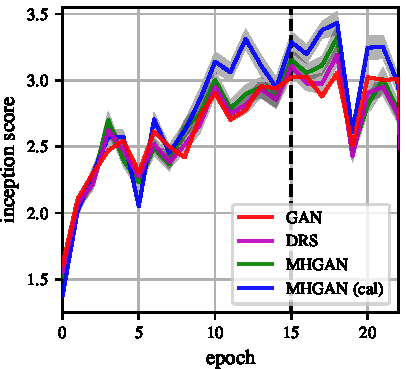
\includegraphics[width=1.8in]{figures/per_epoch.pdf}
       \caption{performance by epoch}
       \label{fig:incep_by_epoch}
    \end{subfigure}
    \begin{subfigure}[b]{0.32\textwidth}
       \centering
       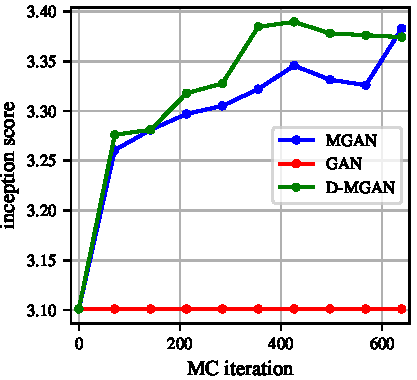
\includegraphics[width=1.8in]{figures/plot_per_mh.pdf}
       \caption{performance by MCMC iteration}
       \label{fig:incep_by_iter}
    \end{subfigure}
    \begin{subfigure}[b]{0.32\textwidth}
       \centering
       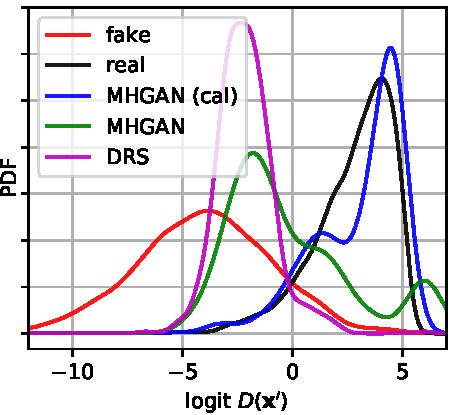
\includegraphics[width=1.8in]{figures/score_dist_overlap.pdf}
       \caption{epoch 13 scores}
       \label{fig:score_dist_overlap}
    \end{subfigure}
    \caption{{\small
    Results of the MH-GAN experiments on CIFAR-10 using the DCGAN\@.
    On the left, we show the inception score by training epoch of the DCGAN at $K=640$.
    MH-GAN denotes using the raw discriminator scores and ``MH-GAN (cal)'' for the calibrated scores.
    The error bars on MH-GAN performance (in gray) are computed using a t-test on the variation per batch across 80 splits of the inception score.
    In the center we show the inception score vs.~MCMC iteration $k$ for the GAN at epoch 15.
    On the right, we show the scores at epoch 13 where there is some overlap between the scores of fake and real images.
    When there is overlap, the MH-GAN corrects the $\PG$ distribution to have scores looking similar to the real data.
    DRS fails to fully shift the distribution because 1)~it does not use calibration and 2)~its ``$\gamma$ shift'' setup violates the validity of rejection sampling.
    }}
\end{figure}

\section{Results}
\label{sec:Results}

For experiments we considered the CelebA~\citep{Liu2015} and CIFAR-10~\citep{Torralba2008} data sets modeled using the DCGAN~\citep{Radford2015} and WGAN~\citep{Arjovsky2017}.
%We also show the results of the calibration statistic $Z$ from~\eqref{eq:calib score}.
%These results confirm our expectation that the raw discriminators do not output well calibrated probabilities.
To evaluate the generator $G'$, we plot inception scores~\citep{Salimans2016} per epoch in Figure~\ref{fig:incep_by_epoch} after $K=640$ MCMC iterations.
The actual performance boost realized by MH-GAN oscillates from one epoch to the next, perhaps because the amount $D$ is ahead or behind changes per epoch.
Because GAN training is a game of sorts, how far ``ahead'' $D$ is will vary by epoch.
Accordingly the statistical significance of the boost from $G$ to $G'$ with calibration varies from no significant change to boost with \smash{$p < 10^{-4}$}.
Figure~\ref{fig:incep_by_iter} shows inception score per MCMC iteration:
Most gains are made in the first $k=100$ iterations, but smaller gains continue to $k=400$.

In Table~\ref{tbl:inception}, we summarize performance (inception score) across all experiments, running MCMC with $K=640$ iterations in all cases.
Behavior is qualitatively similar to that in Figure~\ref{fig:incep_by_epoch}.
While DRS improves on a direct GAN, MH-GAN improves inception score more in every case.
Calibration helps in every case.
There was not a substantial difference between different calibration methods, but we found a slight advantage for isotonic regression
Results are computed at epoch 60, as in Figure~\ref{fig:incep_by_epoch} error bars and p-values are computed using a paired t-test across inception score batches, and all results are significantly better than the baseline GAN at \smash{$p < 0.05$}.

\begin{table}[htbp]
\begin{center}
  \caption{{\small
    Results showing inception score improvements from MH-GAN on DCGAN and WGAN at epoch 60.
    Like Figure~\ref{fig:incep_by_epoch}, the error bars and p-values are computed using a paired t-test across inception score batches.
    All results except for DCGAN on celebA all significant at \smash{$p < 10^{-4}$}.
    WGAN does not learn a typical GAN discriminator that outputs a probability, so calibration is actually required in this case.
    }}
    \label{tbl:inception}
{\scriptsize
\begin{tabular}{|l|l|r|l|r||l|r|l|r|}
\toprule
~                 & \multicolumn{4}{c||}{DCGAN}                               & \multicolumn{4}{c|}{WGAN} \\
\toprule
~            & {CIFAR-10}                &      p   & CelebA                  &      p   & CIFAR-10                 &       p  & CelebA                 &       p  \\
\midrule
%\hline \\
GAN          &        2.8789             &       -- &      2.3317             &       -- &       3.0734             &       -- &     2.7876             &       -- \\
DRS          &        2.977(77)          &   0.0131 &      2.511(50)          &  <0.0001 &               ~          &        ~ &             ~          &        ~ \\
DRS (cal)    &        3.073(80)          &  <0.0001 &      2.869(67)          &  <0.0001 &       3.137(64)          &   0.0497 &     2.861(66)          &   0.0277 \\
MH-GAN       &        3.113(69)          &  <0.0001 &      2.682(50)          &  <0.0001 &               ~          &        ~ &             ~          &        ~ \\
MH-GAN (cal) &        \textbf{3.379}(66) &  <0.0001 &      \textbf{3.106}(64) &  <0.0001 &       \textbf{3.305}(83) &  <0.0001 &     \textbf{2.889}(89) &   0.0266 \\
\bottomrule
\end{tabular}
}
\end{center}
\end{table}

% Removed uncalibrated for WGAN since it makes no sense:
%2.807(81) &  <0.0001 &     3.036(79) &  <0.0001
%3.130(70) &   0.1080 &     2.865(88) &   0.0827

In Figure~\ref{fig:score_dist_overlap}, we visualize what $G'$ does to the distribution on discriminator scores.
MCMC shifts the distribution of the fakes to match the distribution on true images.

Additionally, to test GAN calibration, we found the $Z$ statistic for the raw discriminator $D$ varies from $-77.57$ to $48.98$ in the first 60 epochs; even after Bonferroni correction at $N \!\!=\!\! 60$ we expect $|Z| < 3.35$ with 95\% confidence for a calibrated classifier.
The calibrated discriminator varies from $-2.91$ to $3.60$, which shows it is almost perfectly calibrated.
Unsurprisingly, it significantly boosts performance in the MH-GAN\@.

\section{Conclusions}
\label{sec:conclusions}

% Usual wrap up BS paragraph
We have shown how to incorporate the knowledge in the discriminator $D$ into an improved generator $G'$.
Our method is based on the premise that $D$ is ``ahead'' of $G$.
The principled MCMC setup selects among samples from $G$ to correct biases in $G$.
We have shown the raw discriminators in GANs are poorly calibrated.
To our knowledge, this is the first time research has evaluated the discriminator in this way.
This is the first work to rigorously show the poor calibration of the discriminator.
The MH-GAN has great potential for extension.

\bibliographystyle{abbrvnat}
\bibliography{mgan_refs} % References file

\end{document}

